\documentclass[11pt,a4paper]{article}
\usepackage[margin=2.5cm]{geometry}
\usepackage{booktabs,hyperref,natbib,graphicx,listings,xcolor,amsmath,microtype,parskip,multirow,caption}
\definecolor{SkyBlue}{HTML}{56B4E9}
\definecolor{Goldenrod}{HTML}{E69F00}
\definecolor{LimeGreen}{HTML}{009E73}
\setlength{\parskip}{6pt}
\usepackage{tikz}
\usetikzlibrary{shapes,arrows,positioning,fit}
\lstset{basicstyle=\ttfamily\small,backgroundcolor=\color{gray!10},frame=single,breaklines=true}
\captionsetup{justification=raggedright,singlelinecheck=false}

% Keywords (used for HAL.science deposit metadata)
\newcommand{\keywords}{prompt repetition, LLM agents, agentic pipelines, ceiling effects, null results, instruction design, pre-registered experiment, multi-step agents, rubric design, token efficiency}
\definecolor{darkblue}{rgb}{0,0.08,0.45}
\hypersetup{
  pdftitle={Ceiling Effects and Convergence: Null Results for Instruction Repetition in LLM-Agent Pipelines},
  pdfauthor={Hugues Clouatre; Amadou Diogo Barry},
  pdfsubject={LLM Agents; Experimental Methods; Null Results},
  pdfkeywords={\keywords},
  colorlinks=true,
  linkcolor=darkblue,
  citecolor=darkblue,
  urlcolor=darkblue,
  filecolor=darkblue,
}
\begin{document}
\hrule height 4pt
\vskip 4mm
\begin{center}
{\LARGE\bfseries Ceiling Effects and Convergence: Null Results\\for Instruction Repetition in LLM-Agent Pipelines\par}
\vskip 4mm
\hrule height 1pt
\vskip 5mm
\small
\begin{minipage}[t]{0.44\textwidth}
\centering
\textbf{Hugues Clouâtre}\\[4pt]HEC Montréal\\\texttt{hugues.clouatre@hec.ca}
\end{minipage}
\hfill
\begin{minipage}[t]{0.54\textwidth}
\centering
\textbf{Amadou Diogo Barry}\\[4pt]Institut national de la recherche scientifique (INRS)\\\texttt{amadoudiogo.barry@inrs.ca}
\end{minipage}
\normalsize
\end{center}
\vskip 8mm

\begin{abstract}
\vspace{3mm}
\textbf{Context:} Prompt repetition, the verbatim duplication of an input transforming
\texttt{<QUERY>} into \texttt{<QUERY><QUERY>}, has been shown to improve accuracy for
non-reasoning large language models on retrieval and multiple-choice benchmarks.
\textbf{Objective:} We ask whether applying this analogous pattern to fixed delegate
instructions produces similar gains in multi-step agentic pipelines.
\textbf{Method:} Three pre-registered controlled experiments used Claude Haiku 4.5 delegates
($n{=}5$ per condition, temperature 0.5) assigned either a single-copy or a repeated-prompt
instruction under blinded binary rubric scoring, totalling 30 sessions and 3,196 messages.
\textbf{Results:} Experiment~1 (session-ID refactoring, 6 criteria) yielded a non-significant
score delta of $+0.30$ with five of six criteria saturated at 100\% in both groups
(Fisher's $p{=}1.000$).
Experiment~2 (tree-sitter scanner evaluation, 7 criteria) produced a complete ceiling effect:
all 10 runs scored 7/7 (Mann-Whitney $U{=}12.5$, $p{=}1.000$).
Experiment~3 (Kotlin grammar synthesis, 7 criteria) revealed rubric-runner co-design failure:
three of seven criteria scored 0/1 across both groups because the required investigations were
absent from the runner prompt. On four reachable criteria, control scored a mean of 2.00/4
and treatment scored 2.40/4 ($U{=}15$, $p{=}0.607$).
Across all three pilot experiments, we detect no effect of prompt repetition on task success.
Treatment agents used 30.6\% fewer total tokens in Exp1 but 7.2\% and 19.9\% more in Exp2--3;
the direction reverses with session length, as long sessions save turns while short sessions pay pure overhead.
\textbf{Conclusion:} Criteria requiring investigations absent from the runner prompt
are unreachable by both groups and must be resolved before effect sizes are interpretable.
\end{abstract}

\vspace{4mm}

\section{Introduction}

\citet{leviathan2025} demonstrated that verbatim repetition of the input, transforming
\texttt{<QUERY>} into \texttt{<QUERY>\allowbreak<QUERY>}, improves accuracy for
non-reasoning large language models across a wide range of benchmarks. The intervention wins 47 of 70
benchmark-model combinations with zero losses, gaining up to 76 pp on positional
retrieval tasks such as NameIndex.
The mechanism is efficient: repeated tokens produce no additional output and impose
no mandatory latency penalty on most providers.

Multi-step LLM-agent pipelines constitute a structurally different evaluation setting.
Agents execute multi-step tool-call loops, accumulate context across hundreds of messages,
and produce structured artifacts graded against binary rubrics.
Whether applying the analogous repetition to fixed delegate instructions produces similar gains
in multi-step agentic pipelines remains untested.

The publicly available AIDev dataset \citep{li2026aidev} captures approximately one million
agent-authored pull requests from real-world GitHub repositories; our study complements this
observational corpus with a controlled laboratory design that enables causal inference over a
single variable (instruction repetition) while holding task, model, and temperature constant.

Three pre-registered controlled experiments address that gap.

\textbf{RQ:} Does prompt repetition (the duplicate-query pattern applied to delegate instructions) improve task success rates in multi-step LLM-agent pipelines?

This is the paper's confirmatory, pre-registered question \citep{kitchenham2002guidelines}. Because repeating an instruction changes prompt length, we additionally track token and message efficiency as an exploratory secondary measure in every experiment. Analysis of Experiment~3 also surfaced a distinct evaluation failure mode, rubric-runner co-design failure, characterized in \S\ref{sec:discussion} as an exploratory finding rather than a pre-specified question.

This paper contributes a null result across three pre-registered experiments, a formal characterization of \emph{rubric-runner co-design failure} as a distinct evaluation failure mode in which rubric criteria are structurally unreachable from the runner prompt, and an open dataset of session logs, scoring justifications, and label-map timestamps archived at \href{https://doi.org/10.5281/zenodo.19696593}{DOI:10.5281/zenodo.19696593} \citep{clouatre2026dataset}, enabling replication and secondary analysis. Negative results remain rare in software engineering research despite explicit calls to value them \citep{paige2017negative}. Absent published null results, a positive finding in one setting risks being generalized without evidence to settings where it has not been tested \citep{wieringa2015generalizing}; we report this null result to constrain that generalization rather than as a preliminary finding awaiting a positive follow-up.

This work addresses topics from the Empirical Software Engineering Special Issue on Agentic Software Engineering: failure patterns in agentic systems (rubric-runner co-design failure), and testing and evaluation of AI agents (pre-registered rubric scoring pipeline).

\section{Related Work}


Independently, \citet{qian2026} show that benchmark saturation varies sharply by task: MATH-500
reaches a discriminability score of 0.16 while AIME 2024 reaches 0.74, showing ceiling effects
suppress treatment signals regardless of intervention strength.
\citet{chen2026causal} show, via causal prompt optimization, that near-ceiling queries produce no detectable treatment signal regardless of prompt quality; all gains concentrate on hard queries. This mirrors Experiments~1 and~2: below the discriminability threshold, outcome variance is too low for any intervention to register.

\citet{zheng2023} establish LLM-as-judge as a practical but validity-limited approach, recommending
inter-rater reliability measures, and report over 80\% agreement between GPT-4
judgments and human preferences on MT-Bench, but note position bias. \citet{shen2023} find single-judge agreement with human raters ranges from
$\kappa{=}0.3$ to $\kappa{=}0.7$ depending on task type \citep{hashemi2024llmrubric}.
The MSR~2026 Mining Challenge applied AIDev to characterise agent failure taxonomies, task-stratified acceptance, and review effort \citep{failureMSR2026,comparingMSR2026,revieweffortMSR2026}; none of these observational studies isolates instruction repetition as a controlled pre-registered independent variable.
The present experiments use a single Haiku~4.5 judge; inter-rater reliability was validated in \S\ref{subsec:scoring-validation}.
\citet{adaptorch2026} show that static parallel agent topologies
achieve competitive results on SWE-bench Verified under greedy decoding, supporting the
delegate design used here. Substantive null results from sound designs are distinct from
methodological failures \citep{sculley2018}: a sound design delimits
intervention scope; a flawed design reveals evaluation infrastructure defects.

\section{Experimental Design}

\subsection{Architecture}

All experiments used the Goose agent framework \citep{goose}. The orchestrator spawned 10 async delegates (5 control, 5 treatment); treatment delegates received instructions repeated verbatim.

\begin{figure}[h]
\centering
\captionsetup{labelformat=empty,justification=raggedright,singlelinecheck=false}
\caption{\small \textbf{Code Snippet 1.} Agent configuration used across all three experiments.}
\label{lst:config}
\begin{lstlisting}
orchestrator:
  model: claude-sonnet-4-6
  provider: gcp_vertex_ai
  temperature: 0.3
  framework: Goose

delegates:
  model: claude-haiku-4-5
  provider: gcp_vertex_ai
  temperature: 0.5
  count_per_experiment: 10  # 5 control, 5 treatment
  extensions: [developer, context7, brave_search]

treatment:
  method: verbatim_repetition  # instructions repeated x2
  control_lengths_chars: [3805, 3399, 3800]  # exp1, exp2, exp3
\end{lstlisting}
\end{figure}

\begin{figure}[h]
\centering
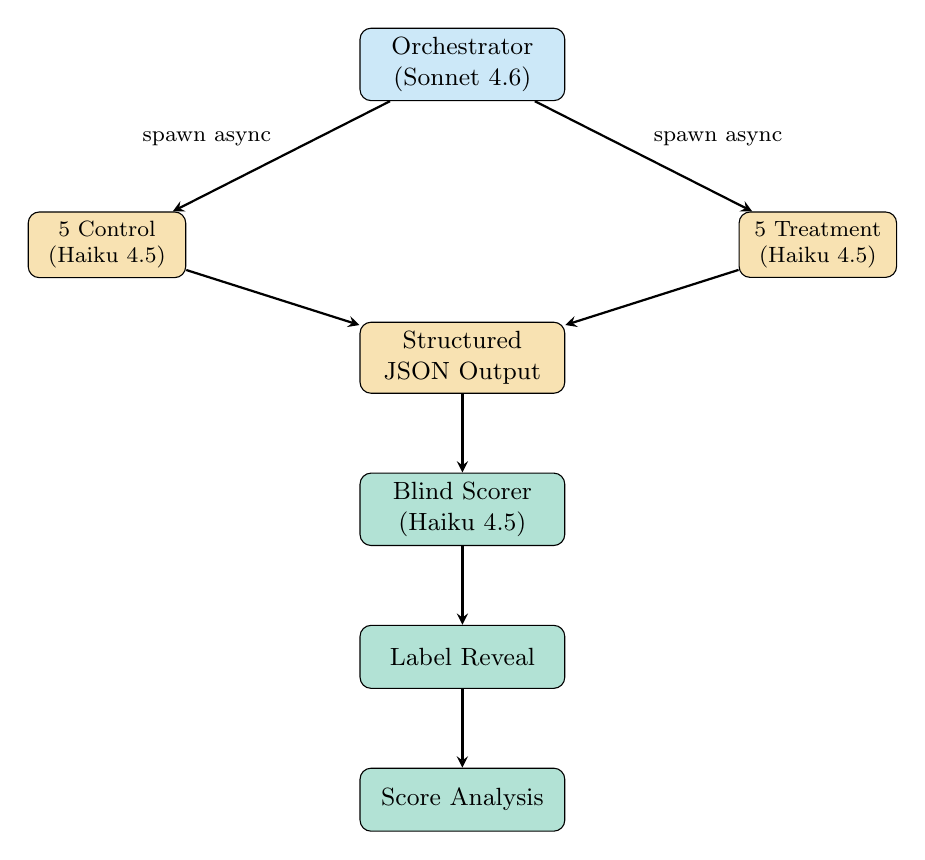
\begin{tikzpicture}[
  node distance=1.0cm and 1.4cm,
  box/.style={rectangle, draw, rounded corners, minimum width=2.6cm, minimum height=0.8cm, align=center, font=\small},
  smallbox/.style={rectangle, draw, rounded corners, minimum width=2.0cm, minimum height=0.7cm, align=center, font=\footnotesize},
  arrow/.style={->, >=stealth, thick}
]
  \node[box, fill=SkyBlue!30] (orch) {Orchestrator\\(Sonnet 4.6)};
  \node[smallbox, below left=1.4cm and 2.2cm of orch, fill=Goldenrod!30] (ctrl) {5 Control\\(Haiku 4.5)};
  \node[smallbox, below right=1.4cm and 2.2cm of orch, fill=Goldenrod!30] (trt) {5 Treatment\\(Haiku 4.5)};
  \node[box, below=2.8cm of orch, fill=Goldenrod!30] (json) {Structured\\JSON Output};
  \node[box, below=1.0cm of json, fill=LimeGreen!30] (scorer) {Blind Scorer\\(Haiku 4.5)};
  \node[box, below=1.0cm of scorer, fill=LimeGreen!30] (reveal) {Label Reveal};
  \node[box, below=1.0cm of reveal, fill=LimeGreen!30] (analysis) {Score Analysis};

  \draw[arrow] (orch) -- node[above left, font=\footnotesize]{spawn async} (ctrl);
  \draw[arrow] (orch) -- node[above right, font=\footnotesize]{spawn async} (trt);
  \draw[arrow] (ctrl) -- (json);
  \draw[arrow] (trt) -- (json);
  \draw[arrow] (json) -- (scorer);
  \draw[arrow] (scorer) -- (reveal);
  \draw[arrow] (reveal) -- (analysis);
\end{tikzpicture}
\caption{\small \textbf{Blinded evaluation pipeline.} The orchestrator spawns 10 independent delegates per experiment.
The blind scorer receives only output JSON and the rubric; group labels are revealed after all
scoring is complete.}
\label{fig:pipeline}
\end{figure}

The treatment mirrors the \texttt{<QUERY><QUERY>} pattern of \citet{leviathan2025} applied to
the delegate system prompt rather than to a single-turn query (Figure~\ref{fig:pipeline}). Goose versions 1.25.0 (Exp1,
Exp2) and 1.31.1 (Exp3) were used. The provider was Vertex AI for all primary runs, with
Amazon Bedrock as a fallback for stream-decode errors in Exp3. The full control instruction template is reproduced in Appendix~\ref{app:control-prompt}.

\subsection{Pre-registration Protocol}
\label{sec:preregistration}

The evaluation rubric was locked before any delegate was spawned. Group assignments were sealed
in a \texttt{label-map.json} file before scoring began, with file creation timestamps serving
as the pre-registration record, archived in the supplementary dataset \citep{clouatre2026dataset}.

A separate Haiku~4.5 instance performed blind scoring:
it received only the delegate output JSON and the rubric criteria. No group labels, run
metadata, or other outputs were visible during scoring.

\subsection{Scoring Validation}
\label{subsec:scoring-validation}

To assess the reproducibility of the rubric scores prior to journal submission, a second LLM judge (Claude Sonnet~4.6) re-scored a stratified sample of 5 sessions using the identical rubric prompts employed by the primary judge (Claude Haiku~4.5). The sample included one control and one treatment session from Experiment~1 (FastMCP refactor), one from each condition in Experiment~2 (Tree-sitter AST), and one treatment session from Experiment~3 (Kotlin grammar). Per-criterion agreement between the two judges was 100\% ($\kappa = 1.00$, 33 criteria across 5 sessions). Session-level pass/fail agreement was also 100\%, though Cohen's $\kappa$ was undefined because all sessions were rated as passing the 50\% threshold by both judges. The per-criterion $\kappa$ of 1.00 indicates almost perfect agreement by Landis--Koch standards~\cite{landis1977}. The Exp2 ceiling effect (all criteria at 100\% in every session) contributed to perfect agreement on those 14 criteria, but the two judges also agreed on all 19 non-ceiling criteria in Experiments~1 and~3, suggesting the rubric is sufficiently well-specified to produce reproducible scores.

The inferential test (Mann-Whitney U, two-tailed, $\alpha{=}0.05$) and effect size metric
(rank-biserial $r$ via \citep{kerby2014}) were pre-specified from Exp2 onward. For Exp1, Fisher's exact test was used post-hoc when the valid-run count fell to $n{=}4$ control and $n{=}5$ treatment.



\paragraph{Statistical power.}
At $n{=}5$ per group, Mann-Whitney U achieves 80\% power only for near-complete separation
effects ($r \geq 0.80$, equivalent to one group dominating the other by 4:1 or more).
Detecting a medium effect ($r{=}0.50$) requires $n \approx 20$ per group \citep{faul2007}.
Infrastructure cost constrained the sample size to 5 runs per group; the experiments are therefore best
interpreted as pilot studies capable of detecting large effects or complete separations, not
medium effects.

\subsection{Experiments}

Each experiment targeted an open, unimplemented GitHub issue as the task source, ensuring no published solution existed (see Table~\ref{tab:experiments}).

\begin{table}[h]
\centering
\caption{\small \textbf{Experiment overview.} Three experiments by task type, rubric width, and valid-run count. Exp1 lost one
control run to session drift; Exp3 includes three provider-retry replacements.}
\label{tab:experiments}
\begin{tabular}{lllll}
\toprule
Exp & Task & Criteria & Valid runs & Task type \\
\midrule
1 & FastMCP session ID refactor & 6 & 9 & Source analysis \\
2 & Tree-sitter AST scanner & 7 & 10 & Code synthesis \\
3 & Kotlin grammar synthesis & 7 & 10 & Code synthesis \\
\bottomrule
\end{tabular}
\end{table}

Experiment~1 targeted issue \texttt{math-mcp-learning-server\#222}, a read-only source
analysis task: characterise a FastMCP session ID refactor. One control run drifted at 93
messages producing no output; excluded, yielding $n{=}4$ valid runs. Experiment~2 targeted
\texttt{aptu\#737}, a code synthesis task evaluating a tree-sitter AST scanner. All 10 runs
produced valid output. An undocumented concurrency cap split Exp2 into two batches (see \S\ref{sec:infrastructure}).
\label{sec:infrastructure}

Experiment~3 targeted issue \texttt{aptu-coder\#649}, a code
synthesis task requiring deep inspection of Kotlin grammar ABI compatibility, node kind
taxonomy, and struct fields. Three runs fell back to Bedrock; all produced output and were included.

\section{Results}
\label{sec:results}

\subsection{Pre-analysis Amendments}
\label{sec:amendments}

After scoring was complete, criteria C1, C5, and C6 each scored 0/1 across both groups in
Experiment~3. Inspection of the runner prompt (\texttt{runner-prompt.md}) confirmed that it
contained no instruction directing agents to investigate ABI compatibility between
\texttt{tree-sitter-kotlin} 0.3.8 and \texttt{tree-sitter} 0.26.6 (C1), to write test cases
exercising \texttt{.kts} file parsing (C5), or to inspect the \texttt{LanguageInfo} struct
fields or \texttt{aptu-coder}\#649 to determine whether a \texttt{DEFUSE\_QUERY} constant was required (C6).

Both groups scored identically (0/1) on C1, C5, and C6, so excluding them cannot bias the treatment comparison in either direction. The exclusion was determined after scoring but before any group labels were inspected, aligning with pre-registration amendment practice \citep{wohlin2012}. All three criteria are retained in the full rubric table (see Appendix~\ref{app:rubrics}); the primary comparison is restricted to C2, C3, C4, and C7.

\subsection{Task Success}

To address the RQ, we compare task success rates between control and treatment groups.

Experiment~1 used Fisher's exact test (see \S\ref{sec:preregistration}); Mann-Whitney columns are shown for consistency. Experiment~2 produced a complete ceiling effect:
all ten runs scored 7/7, rendering the test uninformative ($U{=}12.5$, $p{=}1.000$,
$r{=}\text{n/a}$).\footnote{$\dagger$ Effect size undefined; all runs scored identically.}
Experiment~3 revealed rubric-runner co-design failure: criteria C1, C5, and C6 scored 0/1
across both groups because the corresponding investigations were absent from the runner prompt.
The restricted analysis retaining only criteria C2, C3, C4, and C7 yields identical rank
ordering and $p$-value to the full-rubric analysis (control mean 0.500, treatment mean 0.600,
on the 0--1 normalized scale). Across all seven criteria, the full-rubric means are control
0.286 and treatment 0.343; the gap between full-rubric and restricted means confirms a
rubric-runner co-design failure rather than a treatment or capability signal.

\begin{table}[h]
\centering
\caption{\small \textbf{Task success results.} Mann-Whitney U test (two-tailed,
$\alpha{=}0.05$). Exp1 $p$-value is from Fisher's exact test ($n_\text{ctrl}{=}4$).
$\dagger$~Complete ceiling; test is uninformative.
$\ddagger$~Degenerate test ($n{=}4$ vs.\ $n{=}5$, single discriminating criterion).}
\label{tab:results}
\begin{tabular}{llcccccc}
\toprule
Exp & Group & $n$ & Mean score & SD & $U$ & $p$ & $r$ \\
\midrule
1 (6 criteria) & Control   & 4 & 5.50 & 0.58 & \multirow{2}{*}{---$^\ddagger$} & \multirow{2}{*}{1.000$^\ddagger$} & \multirow{2}{*}{$+$0.30} \\
               & Treatment & 5 & 5.80 & 0.45 &     &       &       \\
\addlinespace
2 (7 criteria) & Control   & 5 & 7.00 & 0.00 & \multirow{2}{*}{12.5$^\dagger$} & \multirow{2}{*}{1.000$^\dagger$} & \multirow{2}{*}{$r{=}\text{n/a}$} \\
               & Treatment & 5 & 7.00 & 0.00 &      &       &       \\
\addlinespace
3 (7 criteria) & Control   & 5 & 2.00 & 0.71 & \multirow{2}{*}{15.0} & \multirow{2}{*}{0.607} & \multirow{2}{*}{$-$0.20} \\
               & Treatment & 5 & 2.40 & 0.89 &      &       &       \\
\bottomrule
\end{tabular}
\end{table}

In Experiment~1, five of six criteria reached 100\% pass rate in both groups; only criterion C5
(must-not constraint captured) discriminated between groups: 50\% control, 80\% treatment (see Table~\ref{tab:results}).
In Experiment~2, every criterion reached 100\% in both groups; no discriminating criterion existed.
In Experiment~3, criterion C7 (language identification) reached 100\% in both groups, while
criteria C1, C5, and C6 were structurally unreachable (floor). Criterion C3 (ELEMENT\_QUERY
patterns) achieved 80\% across both groups, indicating agents can perform structured synthesis
when the task is explicitly set.

\subsection{Token and Message Efficiency}

As a secondary, exploratory outcome measure, we compare token and message counts between conditions.

In Experiment~1, treatment agents consumed 30.6\% fewer total tokens than control
(median 1{,}032{,}311 vs.\ 716{,}324); treatment sessions converged in fewer turns (see Table~\ref{tab:efficiency}).
In Experiment~2, treatment agents used 7.2\% more total tokens than control
(median 703{,}993 vs.\ 755{,}144); sessions were already saturated and no turns were eliminated,
so the doubled prompt added net input overhead. In Experiment~3, treatment agents
consumed 19.9\% more total tokens than control (mean 41{,}880 vs.\ 50{,}220); sessions averaged
12 messages with no turns saved, so the doubled prompt imposed pure input overhead with no performance gain.

\begin{table}[h]
\centering
\caption{\small \textbf{Resource usage by experiment and condition.} Token counts are median per-run totals. Latency
is wall-clock seconds from delegate spawn to output file write. Exp1 control excludes the
drift-failure run. Exp3 latency medians exclude runs with provider-retry overhead.}
\label{tab:efficiency}
\begin{tabular}{llccc}
\toprule
Experiment & Condition & Median Total Tokens & Median Messages & Median Latency (s) \\
\midrule
\multirow{2}{*}{Exp1} & Control   & 1{,}032{,}311  & 204.5   & 136 \\
                      & Treatment &   716{,}324    & 138   &  93 \\
\addlinespace
\multirow{2}{*}{Exp2} & Control   & 703{,}993  & 142   & 117 \\
                      & Treatment & 755{,}144  & 142   & 112 \\
\addlinespace
\multirow{2}{*}{Exp3} & Control   &  41{,}880  &  12   &  62 \\
                      & Treatment &  50{,}220  &  12   &  72 \\
\bottomrule
\end{tabular}
\end{table}

\subsection{Per-Criterion Pass Rates}

To characterize the rubric-runner co-design failure identified during analysis (\S\ref{sec:amendments}), we examine per-criterion pass rates.

Fig.~\ref{fig:passrates} displays per-criterion pass rates with Wilson 95\% confidence
intervals. The pattern of near-uniform ceiling saturation in Experiments~1 and~2 contrasts
sharply with the bimodal floor-ceiling structure in Experiment~3.

\begin{figure}[h]
\centering
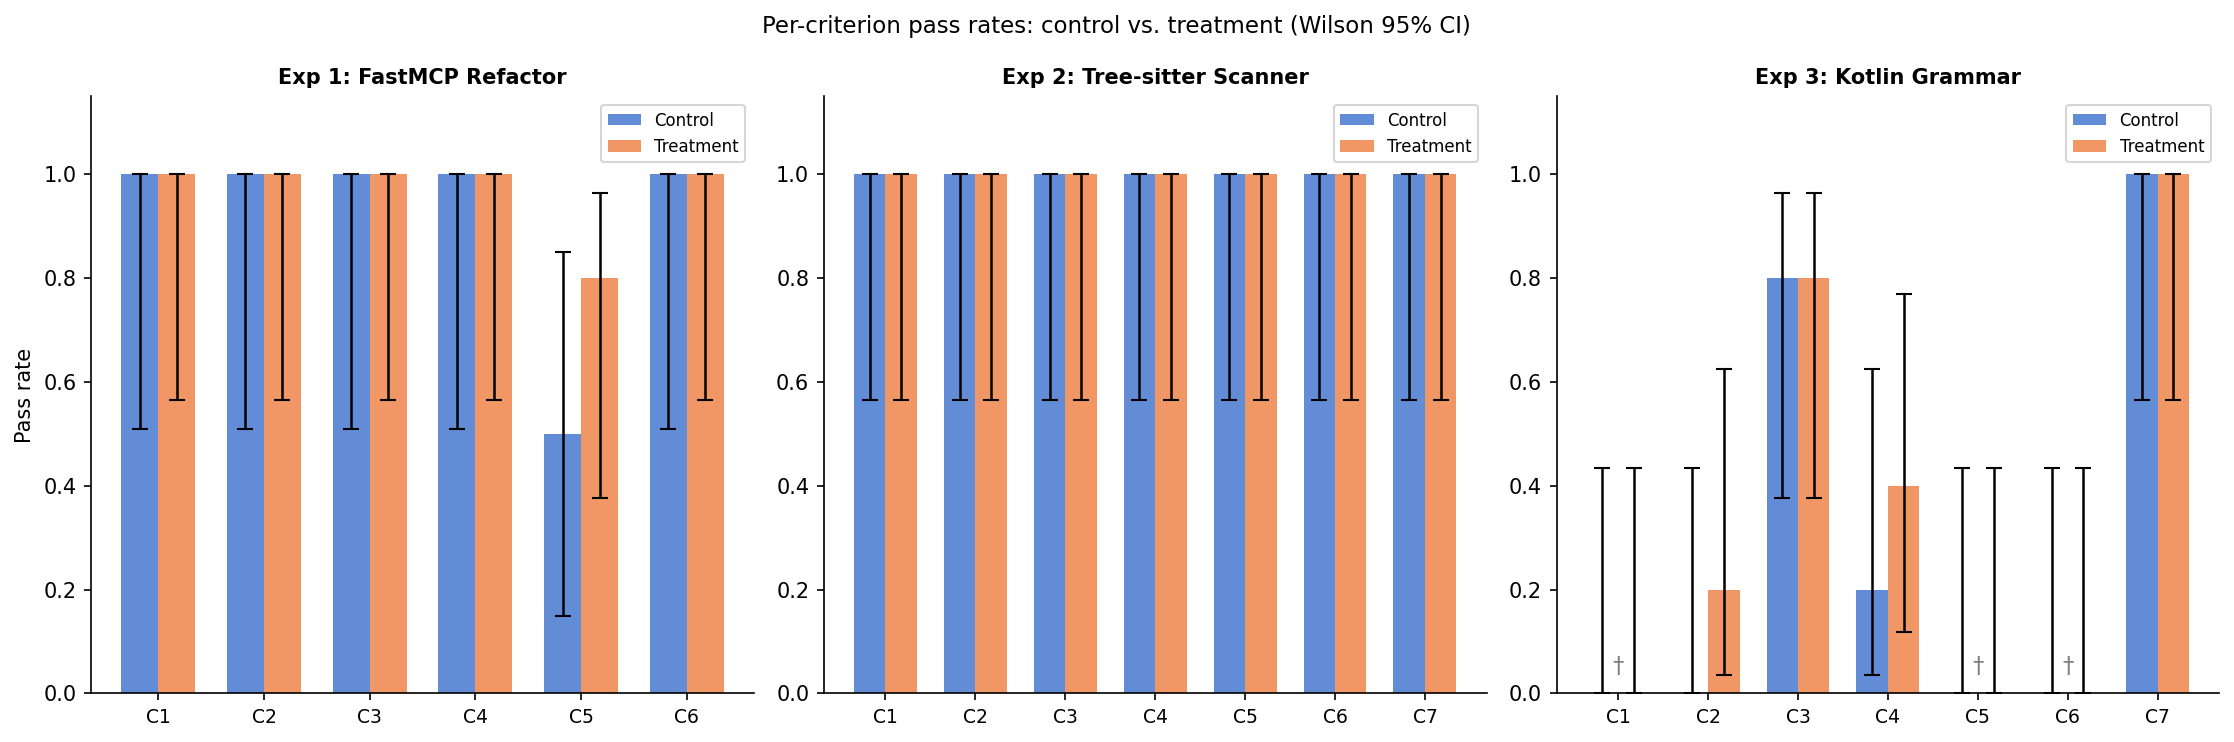
\includegraphics[width=0.9\linewidth]{figures/pass-rates.png}
\caption{\small \textbf{Per-criterion pass rates.} Control vs.\ treatment across all three experiments.
Wilson 95\% confidence intervals shown. Criteria scoring 0/N in both groups are marked with
$\dagger$. (Colors use the Okabe-Ito colorblind-safe palette.)}
\label{fig:passrates}
\end{figure}

Fig.~\ref{fig:tokens} shows token usage by group and experiment.
Experiment~3's reversal, where treatment consumed more tokens despite no
performance gain, illustrates the cost of repeated prefill in short agentic loops.

\begin{figure}[h]
\centering
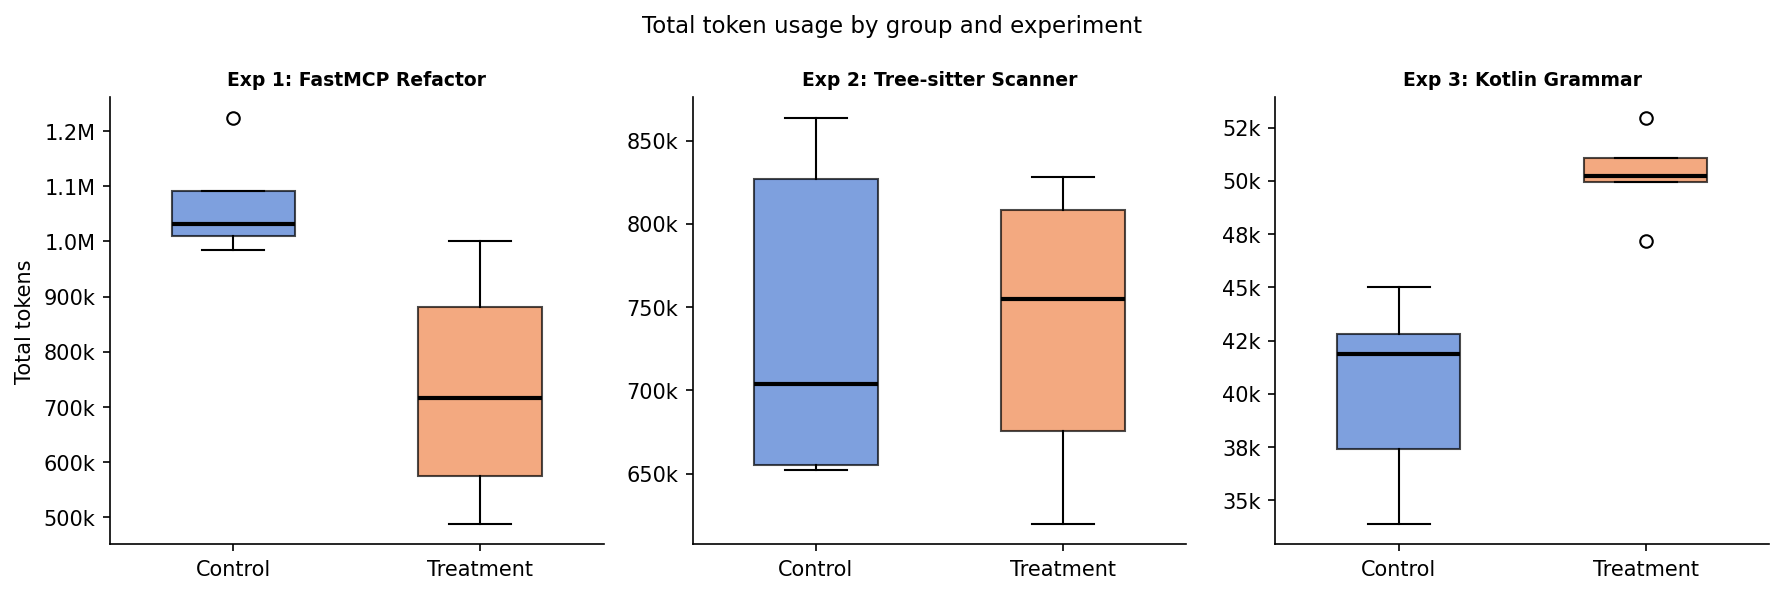
\includegraphics[width=0.9\linewidth]{figures/token-efficiency.png}
\caption{\small \textbf{Token usage by group.} Box plots show median and IQR per experiment. (Colors use the Okabe-Ito colorblind-safe palette.)}
\label{fig:tokens}
\end{figure}

\section{Discussion}
\label{sec:discussion}

\subsection{Mechanism Mismatch}

Prompt repetition enables each token in \texttt{<QUERY>} to attend to every other token in a single causal pass, a mechanism effective only for single-turn inputs where the full context fits in one forward pass; in multi-step loops, the instruction's relative weight dissipates as context grows \citep{leviathan2025}.
By the time agents in Experiments~1 and~2 had exchanged 140--200 messages, the duplicated
instruction constituted a diminishing fraction of total context.

\begin{figure}[h]
\centering
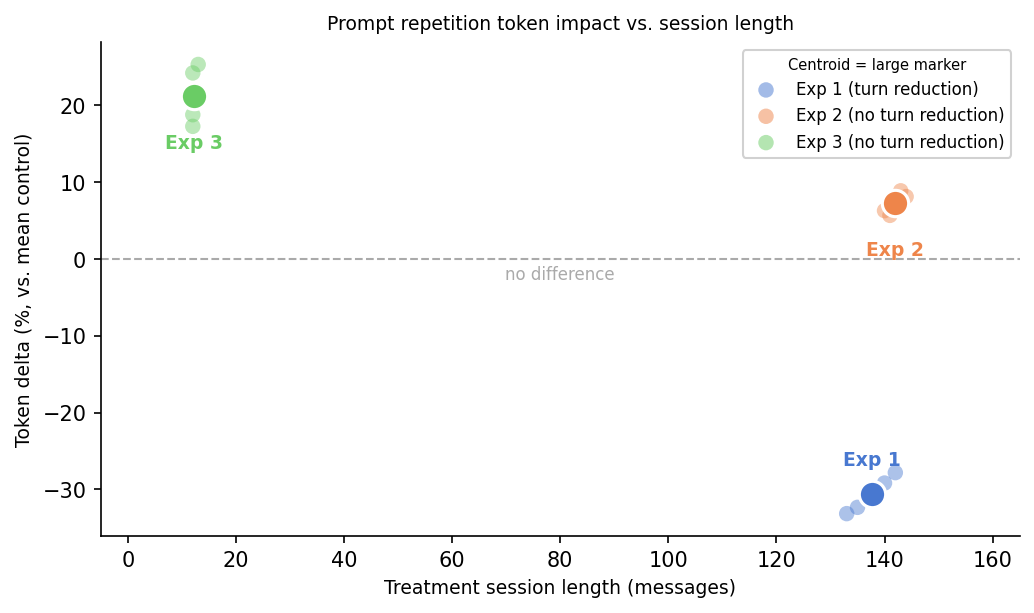
\includegraphics[width=0.85\linewidth]{figures/session-length-crossover.png}
\caption{\small \textbf{Prompt repetition token impact vs.\ session length.} Each point is one experiment; x-axis is mean control session length (messages), y-axis is token delta (\%, treatment vs.\ control), point size scales with mean control token volume. Turn delta is annotated below each point. Token savings require turn reduction; pure overhead accrues when turn count is unchanged. (Colors use the Okabe-Ito colorblind-safe palette.)}
\label{fig:crossover}
\end{figure}

The direction of the token delta is therefore a function of session length: in long-session
experiments, turn savings dominate; in short-session experiments, prompt overhead dominates. (Fig.~\ref{fig:crossover}).

Let $p$ be the prompt token count and $\bar{c}$ the mean tokens per message. A repeated
prompt adds $p$ tokens to every prefill. Each avoided turn eliminates $\bar{c}$ tokens of
accumulated context, where $\bar{c}$ grows with session length. The crossover point $L^*$
satisfies $p = \bar{c}(L^* - 1)$, giving $L^* \approx p/\bar{c} + 1$: sessions longer than
$L^*$ yield a net token saving; sessions shorter than $L^*$ incur overhead. For Experiment~3 ($p \approx 950$, $\bar{c} \approx
3{,}300$ tokens/message), $L^* \approx 1.3$ messages, well below the observed 12-message median.
Yet treatment agents still consumed more tokens, because repeated instructions did not reduce
turn count: agents could not complete structurally unreachable criteria regardless of
instruction emphasis, so the turn-count assumption underlying $L^*$ does not hold under
rubric-runner misalignment.

\subsection{Rubric-Runner Co-design Failure}

A criterion is \emph{structurally unreachable} if no instruction in the runner prompt tasks the corresponding investigation (defined in \S\ref{sec:amendments}). The resulting floor effect is not an agent signal; it is an evaluation design artifact.
Experiment~3 exemplifies this failure mode. Criteria C1, C5, and C6 required agents to inspect
ABI compatibility constraints, node-kind taxonomy sources, and struct field layouts; none of
these investigations appeared in the runner prompt, and both groups scored 0/1 on all three
criteria.

We propose a rubric-runner alignment score $A = k_r / k$ where $k$ is the total number of
rubric criteria and $k_r$ is the number of criteria traceable to at least one explicit
instruction in the runner prompt. For Experiment~3, $A{=}4/7{=}0.57$; for Experiments~1
and~2, $A{=}1.0$. We recommend $A{=}1.0$ as a necessary (though not sufficient)
pre-registration gate: any criterion with $A{<}1.0$ should be revised or removed before
sealing the rubric. This eliminates a class of evaluation failures endemic to LLM-agent pipelines where rubric authors and prompt authors operate independently.

\citet{midolo2026guidelines} derive ten prompt improvement guidelines for code generation via iterative test-driven refinement, finding that explicitly specifying output post-conditions and I/O contracts produces the largest gains in test-pass rates, while structural repetition does not appear among the improvement patterns. This corroborates the rubric-runner alignment principle advanced here: traceability, not repetition count, is the operative lever.

\subsection{Infrastructure Confounds}

The Goose agent framework enforces a concurrency cap via
\texttt{GOOSE\_MAX\_BACKGROUND\_TASKS} (defaults to~5; configurable since Goose
1.29\footnote{\url{https://github.com/aaif-goose/goose/pull/7940}}).
In Experiment~2, this cap silently serialized ten delegates into two batches
approximately four minutes apart, introducing a temporal gap not anticipated in the
pre-registration. This serialization does not affect the statistical conclusion, but it illustrates a broader risk. Researchers should explicitly log concurrency caps and batch boundaries; undocumented serialization can bias latency measurements and, in non-ceiling experiments, interact with task difficulty.

\subsection{Future Work}

Three gaps follow from the present design. First, $n{=}5$ per group is
underpowered for small effects; replication with $n{\geq}20$ and tasks whose
baseline pass rate falls below 0.5 would determine whether prompt repetition
produces any signal once ceiling and floor artifacts are removed. Second,
multi-judge scoring with a reported intraclass correlation coefficient remains
a key validity gap: a single LLM judge cannot detect systematic scorer bias,
and a human--model cross-validation would strengthen internal
validity. Third, all delegates used Haiku 4.5; reasoning models and
larger tiers may exhibit different context-weighting dynamics under prompt
repetition and warrant a dedicated replication.

\section{Threats to Validity}
\label{sec:threats}

\subsection{Construct Validity}

Three aspects of the rubric design threaten construct validity.
First, the rubric-runner co-design failure documented in \S\ref{sec:discussion}---where three of seven criteria in Experiment~3 scored 0/1 because the runner prompt lacked instructions for the required investigations---means those criteria measure runner-prompt completeness rather than agent capability, limiting our ability to conclude that prompt repetition affects criterion-level pass rates on structurally unreachable items.
Second, the binary pass/fail granularity of each criterion compresses within-condition variance, reducing sensitivity to partial improvements that a polytomous or continuous scoring scheme might detect.
Third, scoring stability across alternative rubric phrasings was not tested, which limits our ability to conclude that the observed pass rates are robust to wording variation.

\subsection{Internal Validity}

Several uncontrolled sources of variance limit internal validity.
First, Goose version 1.25.0 was used for Experiments~1 and~2 while version 1.31.1 was used for Experiment~3; version-specific behavioral changes in agent scheduling or tool-handling logic cannot be ruled out as confounds.
Second, two individual runs in Experiment~3 fell back to Bedrock due to Vertex AI rate limits before retrying successfully on Vertex; all token and score data derive from the successful Vertex runs, but the transient provider switch cannot be ruled out as a minor infrastructure variable.
Third, a single LLM judge (Claude Haiku~4.5) performed all rubric scoring with no human calibration; an inter-rater reliability check using a second LLM judge (Claude Sonnet~4.6) across 5 stratified sessions found perfect agreement ($\kappa = 1.00$, see~\S\ref{subsec:scoring-validation}), though the small sample and ceiling effects limit the precision of this estimate, and our ability to conclude that scores are reproducible across non-LLM judges remains limited.
Fourth, task ordering within each session was not randomized or counterbalanced; order effects---fatigue, learning, or context carry-over---are uncontrolled and limit our ability to attribute score differences solely to the treatment.
Fifth, as discussed in \S\ref{sec:discussion}, the \texttt{GOOSE\_MAX\_BACKGROUND\_TASKS} concurrency cap serialized Experiment~2 delegates into two batches; while this did not affect the statistical conclusion in the present ceiling-affected data, it limits our ability to conclude that latency or delegation dynamics were uniform across the experiment.

\subsection{External Validity}

The experimental design constrains external validity along four dimensions.
First, only three software-engineering tasks were sampled (session-ID refactoring, tree-sitter scanner implementation, and Kotlin grammar synthesis), which limits our ability to generalize to the broader distribution of SWE-bench-style tasks or to non-engineering domains such as data analysis or creative writing.
Second, all experiments used a single model (Claude Haiku 4.5) at a single temperature ($0.5$); results may not generalize to reasoning models, larger tiers, or other providers.
Third, a single agentic framework (Goose) was used; framework-specific features such as delegate spawning semantics or context-window boundaries may interact with prompt-repetition effects in ways that limit generalizability to other frameworks such as LangGraph or CrewAI.
Fourth, the controlled lab setting---pre-defined tasks, isolated repositories, and scripted pipeline execution---limits our ability to conclude that the null results hold in production pipelines with variable task difficulty, real-time API failures, and human-in-the-loop interruptions.

\subsection{Conclusion Validity}

Statistical power and design choices constrain conclusion validity.
The sample size of $n{=}5$ per condition was underpowered for medium effect sizes (Cohen's $d \approx 0.5$); the study was powered for large effects only, which limits our ability to conclude that prompt repetition has no practically meaningful effect at smaller effect sizes.
No multiple-comparison correction was applied across the three experiments, inflating the family-wise error rate.
Ceiling effects in Experiments~1 and~2 compress variance and further reduce statistical power, making true effects harder to detect even if they exist.
Finally, Experiment~1 was not fully pre-registered---the statistical test was not pre-specified---which mitigates but does not eliminate the risk of HARKing (hypothesizing after results are known); the partial pre-registration limits our ability to classify all three experiments as confirmatory.

\section{Conclusion}
\label{sec:conclusion}

Three pre-registered controlled experiments find no evidence that prompt repetition improves
task-success rates for LLM agents executing structured software-engineering tasks in multi-step
pipelines. The null results hold across two distinct calibration failure modes: near-ceiling
task difficulty (Experiments~1 and~2) and rubric-runner co-design failure (Experiment~3). The
evidence points instead to rubric-runner alignment as the higher-leverage design investment.
These findings do not extend to the positional-retrieval and multiple-choice settings where
prompt repetition's gains are established.

\section*{Data Availability}

All session logs, scoring records, and pre-registration materials are publicly archived at
\href{https://doi.org/10.5281/zenodo.19696593}{DOI:\allowbreak{}10.5281/zenodo.19696593}
\citep{clouatre2026dataset}.

\bibliographystyle{abbrvnat}
\bibliography{refs}

\clearpage
\appendix
\section*{Appendices}

\section{Control Prompt Template}
\label{app:control-prompt}

The following listing shows the control instruction template, the Scout delegate prompt used in all three experiments.
The treatment condition repeats this block verbatim a second time.

\begin{figure}[h]
\centering
\captionsetup{labelformat=empty,justification=raggedright,singlelinecheck=false}
\caption{\small \textbf{Code Snippet 2.} Control prompt template. The treatment condition appends an identical copy immediately below. Sourced from
\texttt{experiments/exp*/runner-prompt.md}.}
\label{lst:control-prompt}
\begin{lstlisting}[language={},breaklines=true,columns=fullflexible]
# Scout Research Agent

You are a Scout research agent. Your role is to explore the codebase,
gather evidence, and produce a structured JSON research report.

## Instructions

1. Clone or inspect the target repository at the specified commit.
2. Read the issue description in full.
3. Investigate all files relevant to the issue.
4. Consult external documentation (Context7, brave_search) as needed.
5. Write a structured JSON report to the output file specified.

## Output Contract

Write your findings to the path provided by the orchestrator.
The output must be valid JSON matching the rubric schema.
Do NOT summarize; include verbatim excerpts and file paths.

## Extensions Available

- developer: file read/write, shell execution
- context7: library documentation lookup
- brave_search: web search

## Constraints

- Temperature: 0.5
- Model: claude-haiku-4-5
- Provider: Vertex AI (Bedrock fallback on stream-decode error)
- Do not modify any source files.
- Do not open pull requests.
\end{lstlisting}
\end{figure}

\section{Treatment Condition}
\label{app:treatment}

The treatment appends a verbatim copy of Appendix~A with no separator.

\begin{figure}[h]
\centering
\captionsetup{labelformat=empty,justification=raggedright,singlelinecheck=false}
\caption{\small \textbf{Code Snippet 3.} Schematic of treatment condition: control instructions repeated
verbatim a second time.}
\label{lst:treatment-schematic}
\begin{lstlisting}[language={},basicstyle=\ttfamily\small]
[INSTRUCTIONS]
[INSTRUCTIONS]  <- verbatim repeat
\end{lstlisting}
\end{figure}

\bigskip



\section{Per-Run Scores}
\label{app:per-run}

Tab.~\ref{tab:per-run} lists all 30 runs across the three experiments with individual scores.

\begin{table}[h]
\centering
\small
\caption{\small \textbf{All 30 per-run scores.} Exp1 control-1 excluded from analysis (drift
failure). Exp3 C1, C5, C6 scored 0/1 in both groups (rubric-runner co-design failure).}
\label{tab:per-run}
\begin{tabular}{lllrrp{4.5cm}}
\toprule
Run ID & Exp & Condition & Score & Criteria & Notes \\
\midrule
scout-control-1   & 1 & Control   & ---  & 0 & Drift failure; no output \\
scout-control-2   & 1 & Control   & 6/6  & 6 & \\
scout-control-3   & 1 & Control   & 6/6  & 6 & \\
scout-control-4   & 1 & Control   & 5/6  & 6 & \\
scout-control-5   & 1 & Control   & 5/6  & 6 & \\
scout-treatment-1 & 1 & Treatment & 6/6  & 6 & \\
scout-treatment-2 & 1 & Treatment & 5/6  & 6 & \\
scout-treatment-3 & 1 & Treatment & 6/6  & 6 & \\
scout-treatment-4 & 1 & Treatment & 6/6  & 6 & \\
scout-treatment-5 & 1 & Treatment & 6/6  & 6 & \\
\addlinespace
scout-run-01 & 2 & Control   & 7/7 & 7 & \\
scout-run-02 & 2 & Treatment & 7/7 & 7 & \\
scout-run-03 & 2 & Control   & 7/7 & 7 & \\
scout-run-04 & 2 & Treatment & 7/7 & 7 & \\
scout-run-05 & 2 & Control   & 7/7 & 7 & \\
scout-run-06 & 2 & Treatment & 7/7 & 7 & \\
scout-run-07 & 2 & Control   & 7/7 & 7 & \\
scout-run-08 & 2 & Treatment & 7/7 & 7 & \\
scout-run-09 & 2 & Control   & 7/7 & 7 & \\
scout-run-10 & 2 & Treatment & 7/7 & 7 & \\
\addlinespace
scout-run-01 & 3 & Control   & 1/7 & 7 & Logging gap \\
scout-run-02 & 3 & Treatment & 2/7 & 7 & \\
scout-run-03 & 3 & Control   & 3/7 & 7 & \\
scout-run-04 & 3 & Treatment & 2/7 & 7 & Bedrock fallback \\
scout-run-05 & 3 & Control   & 2/7 & 7 & \\
scout-run-06 & 3 & Treatment & 4/7 & 7 & \\
scout-run-07 & 3 & Control   & 2/7 & 7 & \\
scout-run-08 & 3 & Treatment & 2/7 & 7 & \\
scout-run-09 & 3 & Control   & 2/7 & 7 & Bedrock fallback \\
scout-run-10 & 3 & Treatment & 2/7 & 7 & Bedrock fallback; 780s wall time \\
\bottomrule
\end{tabular}
\end{table}

\section{Rubric Criteria}
\label{app:rubrics}

\subsection*{Experiment 1: FastMCP Session ID Refactor (6 criteria)}

\begin{enumerate}
  \item \textbf{C1} Source file 1 identified (\texttt{src/math\_mcp/tools/persistence.py})
  \item \textbf{C2} Source file 2 identified (\texttt{src/math\_mcp/tools/calculate.py})
  \item \textbf{C3} Anti-pattern found (\texttt{id(ctx.lifespan\_context)})
  \item \textbf{C4} Replacement API correct (\texttt{ctx.set\_state} / \texttt{ctx.get\_state}
        with UUID)
  \item \textbf{C5} Must-Not constraint captured (non-serializable values, process-restart
        caveat)
  \item \textbf{C6} FastMCP docs consulted (\texttt{gofastmcp.com/servers/context} or
        equivalent)
\end{enumerate}

\subsection*{Experiment 2: Tree-sitter AST Scanner (7 criteria)}

\begin{enumerate}
  \item \textbf{C1} SecurityScanner implementation file identified; verified against actual
        repo structure, not assumed.
  \item \textbf{C2} Line-by-line regex limitation understood; must reference single-line
        constraint; cite \texttt{aptu}\#735 or \texttt{aptu}\#736 or quote the test.
  \item \textbf{C3} tree-sitter-rust version verified against Cargo.toml or Context7 docs;
        must identify 0.23 (not assumed from issue text alone).
  \item \textbf{C4} Hybrid vs.\ full-migration tradeoff articulated with codebase evidence;
        must name specific patterns or files.
  \item \textbf{C5} At least 2 specific patterns identified as requiring multi-line detection;
        must name actual pattern IDs or descriptions from source code.
  \item \textbf{C6} Data-flow/taint tracking gap noted as unsolved by tree-sitter alone;
        explicit statement that AST traversal does not equal taint analysis.
  \item \textbf{C7} Binary size / grammar crate count estimated with specifics; must name at
        least 3 target languages with their crate names.
\end{enumerate}

\subsection*{Experiment 3: Kotlin Grammar Synthesis (7 criteria)}

\begin{enumerate}
  \item \textbf{C1}$^\dagger$ tree-sitter-kotlin 0.3.8 LANGUAGE export verified and ABI
        relationship with tree-sitter 0.26.6 fully characterized with evidence; incompatibility
        is a valid finding if documented.
  \item \textbf{C2} Kotlin companion object node kind identified as \texttt{object\_declaration}
        with companion modifier; \texttt{delegation\_specifiers} children enumerated
        distinguishing {\ttfamily superclass\_type\_\linebreak[0]with\_constructor} from
        \texttt{user\_type}.
  \item \textbf{C3} At least 3 query patterns from the tree-sitter-kotlin corpus correctly
        captured in \texttt{ELEMENT\_\linebreak[0]QUERY}.
  \item \textbf{C4} \texttt{extract\_inheritance} handler correctly walks
        \texttt{delegation\_specifiers} and separates nodes of kind
        {\ttfamily superclass\_type\_\linebreak[0]with\_constructor} (has argument parens)
        from \texttt{user\_type} (no parens).
  \item \textbf{C5}$^\dagger$ Unit tests confirm \texttt{.kt} AND \texttt{.kts} file parsing
        both work; at least 1 test with \texttt{.kts} syntax.
  \item \textbf{C6}$^\dagger$ \texttt{DEFUSE\_QUERY} constant created for Kotlin if required
        by current \texttt{LanguageInfo} struct, or justified as None if not applicable; must
        cite inspection of \texttt{LanguageInfo} struct fields or \texttt{aptu-coder}\#649.
  \item \textbf{C7} All structural wiring described: feature flag, query constant names,
        \texttt{EXTENSION\_MAP} entries, \texttt{mod.rs} arms, module registered.
\end{enumerate}

\noindent $\dagger$ Excluded from primary treatment comparison (rubric-runner co-design
failure; both groups scored 0/1; see \S\ref{sec:amendments}).

\end{document}
